\documentclass[a4paper,10pt,twoside]{article}

\usepackage[utf8]{inputenc}
\usepackage[IL2]{fontenc}

\usepackage[english]{babel}

\PassOptionsToPackage{table}{xcolor}

\usepackage{amsmath}
\usepackage{amsthm}
\usepackage{mathtools}
\usepackage{amsfonts}
\usepackage{fullpage}
%\usepackage{showframe}
\usepackage{booktabs}
\usepackage{multirow}
\usepackage{dcolumn}
\usepackage{tikz}
\usetikzlibrary{shapes.geometric, arrows, calc, intersections}
\usepackage{subfiles}
%\usepackage[ruled]{algorithm2e}
\usepackage[figuresright]{rotating}
\usepackage[table]{xcolor}
\usepackage{caption}
\usepackage{subcaption}
\usepackage{geometry}
\usepackage{pdflscape}
\usepackage{longtable}
\usepackage{multicol}
\usepackage{rotating}
\usepackage{accents}
\usepackage[ruled,english]{algorithm2e}
\usepackage{hyperref}


\usepackage[capbesideposition=inside,facing=yes,capbesidesep=quad]{floatrow}
\usepackage[maxfloats=25]{morefloats}

%\usepackage{hyperref}



% Theorem Styles
\newtheorem{theorem}{Theorem}[section]
\newtheorem{lemma}[theorem]{Lemma}
\newtheorem{proposition}[theorem]{Proposition}
\newtheorem{corollary}[theorem]{Corollary}
% Definition Styles
\theoremstyle{definition}
\newtheorem{definition}[theorem]{Definition}
\newtheorem{example}[theorem]{Example}
\theoremstyle{remark}
\newtheorem{remark}{Remark}
\newtheorem*{remarkn}{Remark}

\renewcommand{\ring}{\mathbb{Z}\left[\beta\right]}
\newcommand{\field}{\mathbb{Q}(\beta)}
\newcommand{\quasi}[1]{\Sigma(#1)}
\newcommand{\widequasi}[1]{\Sigma\left(#1\right)}
\newcommand{\RN}{\mathbb{R}}
\newcommand{\ZN}{\mathbb{Z}}
\newcommand{\NN}{\mathbb{N}}
\newcolumntype{d}[1]{ D{:}{:}{-1} }

\setlength{\parskip}{0.3em}
\setcounter{tocdepth}{1}


\graphicspath{ {img/} }


\newcommand{\uhat}{\underaccent{\check}}

\newcommand{\uwidehat}[1]{%
  \mathpalette\douwidehat{#1}%
}

\makeatletter
\newcommand{\douwidehat}[2]{%
  \sbox0{$\m@th#1\widehat{\hphantom{#2}}$}%
  \sbox2{$\m@th#1x$}
  \sbox4{$\m@th#1#2$}
  \dimen0=\ht0
  \advance\dimen0 -0.5\ht2
  \dimen2=\dp4
  \rlap{%
    \raisebox{\dimexpr\dimen0-\dimen2}{%
      \scalebox{1}[-1]{\box0}%
    }%
  }%
  {#2}%
}
\makeatother



\begin{document}

%\thispagestyle{empty}

%\begin{center}

%{\Large ČESKÉ VYSOKÉ UČENÍ TECHNICKÉ V~PRAZE} \\[3.5mm]
%{\Large Fakulta jaderná a fyzikálně inženýrská}

%\vspace{\stretch{1}}

%{\Huge\textbf{VÝZKUMNÝ ÚKOL}}

%\vspace{\stretch{1}}

%{\Large \hspace*{1cm} 2016 \hfill Eduard Šubert \hspace*{1cm}}

%\end{center}

%%%%%%%%%%%%%%%%%%%%%%%%%%%%%%%%%%%%%%%%%%%%%%%%%%%%%%%%%%%%%%%%%%%%%%%%%%%%%%%%%%%%%%%%%%%%%%%%%%%
%% TITULNÍ STRANA PRÁCE
\clearpage
\pagestyle{empty}
\cleardoublepage

\thispagestyle{empty}

\begin{center}

{\Large ČESKÉ VYSOKÉ UČENÍ TECHNICKÉ V~PRAZE} \\[3.5mm]
{\Large Fakulta jaderná a fyzikálně inženýrská} \\[3.5mm]
{\Large Katedra matematiky}

\vspace{\stretch{0.75}}

{\Large VÝZKUMNÝ ÚKOL}

\vspace{\stretch{0.5}}

{\LARGE
\textbf{Voronoiova dláždění kvazikrystalů s~dvanáctičetnou symetrií}
\par}

\vspace{1cm}

{\LARGE
\textbf{Voronoi tillings of quasicrystals with dodecagonal symmetry}
\par}

\vspace{\stretch{1.25}}

\end{center}

\begin{tabular}{ll} 
{\Large Author:} & {\Large Eduard Šubert} \\[1mm]
{\Large Supervisor:} & {\Large Ing. Petr Ambrož, Ph.D.} \\[1mm]
{\Large Academic year:}     & {\Large 2015/2016}
\end{tabular}

%%%%%%%%%%%%%%%%%%%%%%%%%%%%%%%%%%%%%%%%%%%%%%%%%%%%%%%%%%%%%%%%%%%%%%%%%%%%%%%%%%%%%%%%%%%%%%%%%%%
%%% ZADÁNÍ PRÁCE

%\clearpage
%\thispagestyle{empty}
%\cleardoublepage

%\thispagestyle{empty}

%\noindent
%{\Large
%Na toto místo přijde svázat \textbf{zadání diplomové práce}!\\
%V~jednom z~výtisků musí být \textbf{originál} zadání, v~ostatních kopie.\par}
%\newpage
%prázdná strana pro zadání
%%%%%%%%%%%%%%%%%%%%%%%%%%%%%%%%%%%%%%%%%%%%%%%%%%%%%%%%%%%%%%%%%%%%%%%%%%%%%%%%%%%%%%%%%%%%%%%%%%%
%%% ČESTNÉ PROHLÁŠENÍ

%\clearpage
\thispagestyle{empty}
\cleardoublepage

\vspace*{\stretch{1}}

\noindent{\bf Čestné prohlášení}

\vspace{0.5cm}

Prohlašuji na tomto místě, že jsem předloženou práci vypracoval samostatně 
a že jsem uvedl veškerou použitou literaturu.

\vspace{1.5cm}

\noindent
\begin{minipage}[b]{5cm}
V~Praze dne \today
\end{minipage}
\hfill
\begin{minipage}[t]{5cm}
\begin{center}
\dotfill\\
Eduard Šubert
\end{center}
\end{minipage}

\vspace*{2cm}

\vspace*{2cm}

%%%%%%%%%%%%%%%%%%%%%%%%%%%%%%%%%%%%%%%%%%%%%%%%%%%%%%%%%%%%%%%%%%%%%%%%%%%%%%%%%%%%%%%%%%%%%%%%%%%
%%% PODĚKOVÁNÍ

\cleardoublepage

\thispagestyle{empty}

\vspace*{\stretch{1}}
\begin{center}\small
Děkuji Ing. Petrovi Ambrožovi, Ph.D. a doc. Ing. Zuzaně Masákové, Ph.D. za pomoc s touto prací.
\end{center}
\vspace*{\stretch{1}}

%%%%%%%%%%%%%%%%%%%%%%%%%%%%%%%%%%%%%%%%%%%%%%%%%%%%%%%%%%%%%%%%%%%%%%%%%%%%%%%%%%%%%%%%%%%%%%%%%%%
%%% CZ/EN ABSTRAKTY A KLÍČOVÁ SLOVA

\cleardoublepage

{
\setlength{\parindent}{0pt}

\textit{Název práce:}
\textbf{Voronoiova dláždění kvazikrystalů s dvanáctičetnou symetrií} \\

\textit{Autor:} Eduard Šubert \\

\textit{Obor:} Matematická informatika \\

\textit{Druh práce:} Výzkumný úkol \\

\textit{Vedoucí práce:}  Ing. Petr Ambrož Ph.D., Katedra matematiky, FJFI ČVUT v~Praze \\

\textit{Abstrakt:} 
Práce se zabývá kvazikrystaly definovanými iracionalitou $2+\sqrt{3}$. Jsou rozebrány jednorozměrné kvazikrystaly především s okny ve tvaru $[c,d)$ a dvourozměrné kvazikrystaly s rovnoběžníkovým oknem i s oknem obecného tvaru. Pro oba případy je studována struktura kvazikrystalů pomocí konstrukce Voronoiova diagramu, nejdříve lokálně a po té globálně. \\

\vspace{1.5cm}

\textit{Title:}
\textbf{Voronoi tillings of quasicrystals with dodecagonal symmetry} \\

\textit{Author:} Eduard Šubert\\

\textit{Abstract:} 
Main focus of the thesis are quasicrystals defined by irrationality $2+\sqrt{3}$. First one-dimensional quasicrystals are analyzed. Next two-dimensional quasicrystals with rhombic window and with a window of a general shape are analyzed also. For each case the structure is investigated with the aid of the Voronoi diagram at first locally and then globally. \\

}

%%%%%%%%%%%%%%%%%%%%%%%%%%%%%%%%%%%%%%%%%%%%%%%%%%%%%%%%%%%%%%%%%%%%%%%%%%%%%%%%%%%%%%%%%%%%%%%%%%%%%
%%% Konec uvodnich stran

\cleardoublepage

\tableofcontents
\setcounter{page}{1}
\cleardoublepage

\section*{Introduction}
\addcontentsline{toc}{section}{Introduction}
Quasiperiodic crystal, or quasicrystal, is a structure that displays some order, however it is not periodic. It fills an infinite space without having a translational symmetry. Qualicrystals however do posses rotational symmetry. 

A lot of research \cite{classification,classificationII,classificationIII} has been done on quasicrystals connected to the irrationality $\tau = \frac{1+\sqrt{5}}{2}$, also known as golden ratio. However there are other irrationalities that give rise to quasicrystal structures \cite{gazeau}: $1+\sqrt{2}$ and $2+\sqrt{3}$. In this work we consider $2+\sqrt{3}$.

Such quasicrystals do have some different properties in comparison with the golden ratio ones, which mostly cause the computational complexity of the algorithms used for analysis to rise significantly. 

The first section covers the essentials for one-dimensional quasicrystals, which are mostly results of a previous work. Next the one-dimensional quasicrystal is fully analyzed and the analysis is applied to a certain subset of two-dimensional quasicrystals. Lastly the results of the analysis of these special two-dimensional quasicrystals are used to analyze a general two-dimensional quasicrystal. 

In the end the bulk of the work is again applied to a different subset of two-dimensional quasicrystals that do exhibit a twelve-fold rotational symmetry. Unfortunately due to the already mentioned rise in computational complexity, these special cases were only studied locally, global analysis will be subject of future work. 
\cleardoublepage
\pagestyle{plain}
\subfile{oneDimension}
%%
%\clearpage
\subfile{twoDimension}
%%
%\clearpage
\subfile{coveringRadiusEstimate}
%%
%\clearpage
\subfile{divisionOfWindow}
%%
%\clearpage
\subfile{catalogRhombusSingle}
%%
%\clearpage
\subfile{catalogRhombusAll}
%%
\cleardoublepage
\subfile{generalWindowFinite}
%%
%\clearpage
\subfile{generalWindowSingle}
%%
%\clearpage
\subfile{generalWindowAll}
%%
%\clearpage
\subfile{circle}
%%
%\clearpage
\subfile{computation}
%%

\clearpage
\pagestyle{empty}
\section*{Conclusion}
\addcontentsline{toc}{section}{Conclusion}
This work presented mostly the theoretical preparation for the analysis of the quasicrystals with a circular window. The analysis is however not yet concluded and so it will be subject of future work. That leaves enough space for a nice quasicrystal with a dodecagonal window which also posses twelve-fold rotational symmetry and also will be a part of the future work. 

\begin{figure}[h!]
\centering
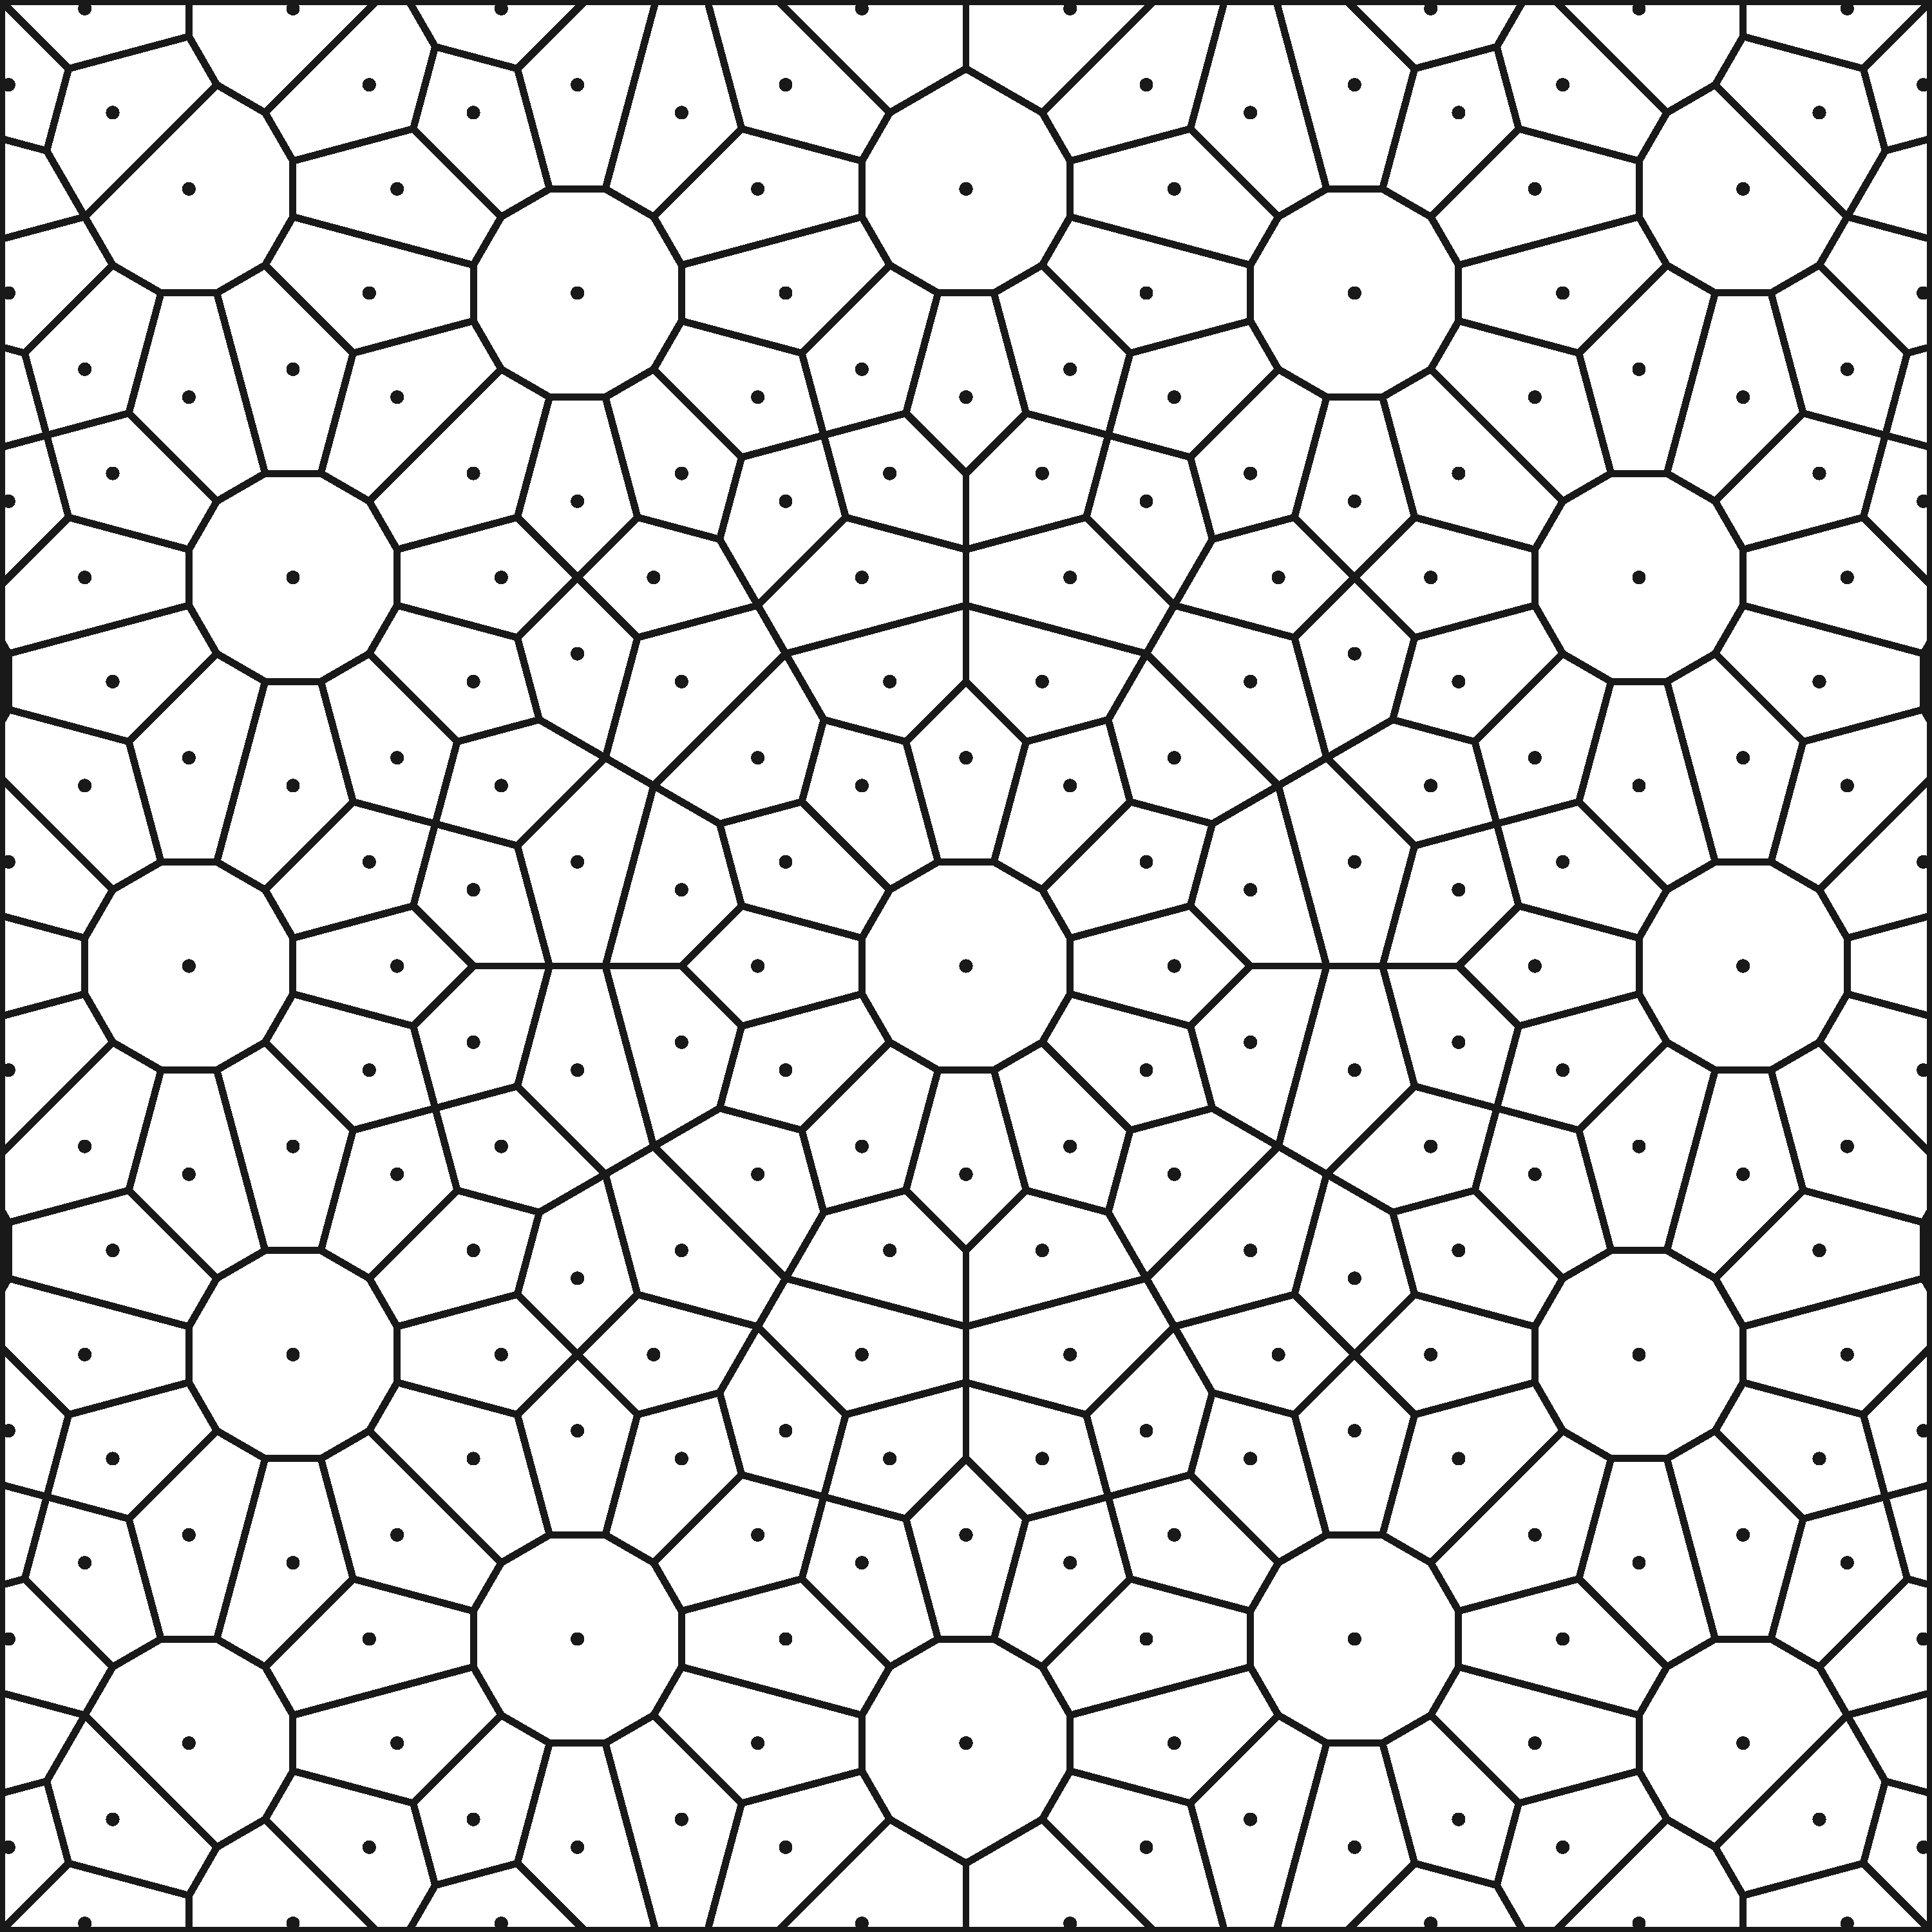
\includegraphics[width=\textwidth]{dodecagon}
\end{figure}

\clearpage
\begin{thebibliography}{9}

\bibitem{classification}
	Z~MASÁKOVÁ, J PATERA a J ZICH. \emph{Classification of Voronoi and Delone tiles in quasicrystals. I. General method.} J. Phys. A \textbf{36} (2003), 1869--1894.

\bibitem{classificationII}
	Z~MASÁKOVÁ, J PATERA a J ZICH. \emph{Classification of Voronoi and Delone tiles of quasicrystals: II. Circular acceptance window of arbitrary size} J. Phys. A \textbf{36} (2003), 1895--1912.

\bibitem{classificationIII}
	Z~MASÁKOVÁ, J PATERA a J ZICH. \emph{Classification of Voronoi and Delone tiles of quasicrystals: III. Decagonal acceptance window of any size} J. Phys. A \textbf{38} (2005), 1847--1960.
  
\bibitem{combinatorial}
	L-S GUIMOND, Z~MASÁKOVÁ, E PELANTOVÁ. \emph{Combinatorial properties of infinite words associated with cut-and-project
 sequences.} J. Théor. Nombres Bordeaux \textbf{15} (2003), 697--725.

\bibitem{gazeau}
	J.-P. GAZEAU. \emph{Pisot-cyclotomic integers for quasilattices} in: The mathematics of long-range aperiodic order (Waterloo, ON, 1995), Kluwer Academic Publishers, Dordrecht, (1997), pp. 175–198.
  
\bibitem{magister}
	J ZICH. \emph{Voronoi \& Delone tiling of quasicrystals}. Fakulta jaderná a fyzikálně inženýrská České vysoké učení technické v~Praze, 2002. Diplomová práce. Vedoucí práce Z~Masáková.

\bibitem{assignment}
	E ŠUBERT. \emph{Voronoiova dláždění a Cut-and-Project množiny}. Fakulta jaderná a fyzikálně inženýrská České vysoké učení technické v~Praze, 2014. Bakalářská práce.
	
\end{thebibliography}
\end{document}
